%\documentclass[a4paper,12pt]{article}
\documentclass[internal]{sintefmemo}
%\documentclass{amsart}
%\usepackage[a4paper, total={17cm, 25cm}]{geometry}

%\usepackage[utf8]{inputenc}
\usepackage[english]{babel}
%\usepackage{amsmath,bm,amsfonts,amssymb}
\usepackage{xcolor}
\usepackage{graphicx}
\usepackage{graphbox} % allows includegraphics[align=c]
\usepackage[round]{natbib}
\usepackage{mathtools}
\usepackage[font=normalsize]{subfig}
\usepackage{float}
\usepackage{hyperref}
\usepackage{xfrac}
%\usepackage{cprotect}%for \verb in captions
%\usepackage{enumerate}
\usepackage{enumitem}
\hypersetup{colorlinks=true,
			linkcolor=blue,
			filecolor=blue,
			urlcolor=blue,
			citecolor=blue}
\newcommand{\mr}{\mathrm}
\newcommand{\mc}{\mathcal}
\let\SSS\S
\renewcommand{\S}{^\mr{S}}
\newcommand{\ii}{\mr{i}\,}
\newcommand{\ee}{\mr{e}}
\let\underscore\_
\renewcommand{\_}[1]{_\mr{#1}}
\newcommand{\oo}[1]{^{(#1)}}
\let\Re\relax
\let\Im\relax
\DeclareMathOperator\Re{Re}
\DeclareMathOperator\Im{Im}
\newcommand{\w}{w}
\newcommand{\bU}{\bm U}
\newcommand{\h}{\hat}
\newcommand{\br}[3]{\left#1#2\right#3}
\newcommand{\rbr}[1]{\left(#1\right)}
\newcommand{\sbr}[1]{\left[#1\right]}
\newcommand{\cbr}[1]{\left\{#1\right\}}
%\newcommand{\bU}{(\nabla\Phi)_{z=\eta}}


\newcommand{\z}{z}
\newcommand{\x}{x}
\newcommand{\y}{y}
\newcommand{\zz}{\zeta}
\newcommand{\xx}{\xi}
\newcommand{\yy}{\sigma}
\newcommand{\kk}{\kappa}

\newcommand{\zmap}{f}
%\newcommand{\zzmap}{\zmap^{-1}}
\newcommand{\zzmap}{\zmap^{\raisebox{.2ex}{$\scriptscriptstyle-1$}}}

%\newcommand{\ww}{w}
%\renewcommand{\w}{\ww^\mr{P}}
\newcommand{\ww}{\omega}
\renewcommand{\w}{w}
%\newcommand{\UU}{\mc U\_p}%
\newcommand{\UU}{\mc U}%
\newcommand{\Jac}{|\zmap_\zz|^2}
\newcommand{\iJac}{|\zmap_\zz|^{-2}}

\newcommand{\surf}{\eta}
%\newcommand{\w}{\varpi}
\newcommand{\dd}{\mr d}
\newcommand{\ddfrac}[2]{\frac{\dd #1}{\dd #2}}

\title{Conformal mapping of bathymetry in the The Higher Order Spectral method}
\author{Andreas H. Akselsen}
\project{302006355-3 (OSC pre-project)}
\date{\today}
\recipient[information]{SINTEF employees}
%\recipient[information,agreed]{Statsbygg}

\begin{document}


%\maketitle
\frontmatter

\tableofcontents

\section{Introduction}
This memo describes the combination of the so-called higher order spectral method (HOS) with a conformal mapping strategy for simulating wave propagation over irregular bathymetry.
The method is fully nonlinear and adheres to no limitations regarding the steepness or severity of bathymetry, also retaining the $\mathcal O(N\log N)$ asymptotic simulation time of the HOS method. 
Only unidirectional wave field are here considered. The method can likely be extended to multidirectional wave fields, although alteration in bathymetry can only occur along one direction.


\section{Conformally mapped bathymetries in the HOS scheme}
We seek to use conformal mapping to project an uneven bathymetry onto a straight line.
Let such a map be described by 
\begin{equation*}
	\z \mapsfrom \zmap(\zz),
\end{equation*}
where $\z = \x+\ii\y$ is the physical plane and $\zz=\xx+\ii\yy$ is the conformal plane. 
The motivation for doing this is that any complex potential 
\begin{equation}
\ww(\zz) = \sum_{j=-\infty}^\infty \h\ww_j \frac{\ee^{\ii \kk_j(\zz+\ii\tilde H)}}{\cosh(\kk_j \tilde H)}; \quad \h\ww_{-j}=\h\ww_{j}^*.
\label{eq:ww}
\end{equation}
in the $\zz$-plane will represent a valid potential $\w[\zmap(\zz)]=\ww(\zz)$ in the physical plane with impermeable kinematics at $\yy=-\tilde H$.
\\



%The complex potential with an impermeable surface at $\yy=0$ is
%\begin{equation}
%\ww(\zz) = \sum_{j=-\infty}^\infty\h\ww_j \frac{\ee^{\ii \kk_j\zz}}{\cosh \kk_j \tilde H}; \quad \h\ww_{-j}=\h\ww_{j}^*.
%\label{eq:ww_logstrip}
%\end{equation}
%$\tilde H$ is a representative depth in the $\zz$-plane introduced to numerically scale $\h\ww_j$.
%
%It is impractical in practice to map a transient free surface within a simulation routine. %, as noted in \autoref{sec:finiteDepth}.
%We can however map $\zz$ to the reference plane $\y = 0$ which is fixed throughout the simulation, and from there use the traditional HOS technique of Taylor expansion.
%Let's call such a mapping $\zz_0(\x)$. It satisfies
%\[
%\z[\zz_0(x)]=x.%\in\mathbb R.
%\]
%Such a map is easily computed numerically using interpolation; the circles in \autoref{fig:SC_step} shows $\z[\zz_0(x)]$ for regularly spaced $x$.
%\\
%
%
%Next we consider the Taylor expansion routine from which the vertical velocity at the free surface is to be determined. 
%This procedure inverts the expansion 
%\[
%\phi\S = \phi(x,h(x)) = \sum_{m=0}^\infty \frac{h^m}{m!}\partial_y^m \phi(x,0)
%\]
%combined with the order expansion 
%\begin{equation}
%\phi=\sum_{n=1}^N\phi\oo n
%\label{eq:phiExpansion}
%\end{equation}
%to get
%\begin{equation}
%\phi\oo{n}(x,0) = 
%\begin{cases}
%\phi\S(x), & n = 1,\\
%- \sum_{m=1}^{n-1} \frac{h^m}{m!}\partial_y^m \phi\oo{n-m}(x,0), & n>1.
%\end{cases}
%\label{eq:phioon}
%\end{equation}
%In terms of the complex potential $\w\oo n(\z)=\phi\oo n(\x,\y)+\ii \psi\oo n(\x,\y)$ we have 
%\begin{equation}
%\partial_y^m \phi\oo{n} = \Re\left\{ \mr{d}_\z^n\w(\z) \ee^{\ii \frac\pi2 n} \right\} .
%\label{eq:ppphi}
%\end{equation}
%It is straightforward to related the derivatives of $\w(\z)$ to the derivatives of $\ww(\zz)$ in \eqref{eq:ww_logstrip} using the derivatives of \eqref{eq:mapSC} and the chain rule. 

Several options from combining conformal mapping with the HOS method are apparent.
Let us list some:
\renewcommand\labelitemi{--}
\begin{enumerate}[label={\roman*)}]
	\item A numerical inverse-mapping approach whereby we map back and forth between the $\z$- and $\zz$-planes at each time step. \label{it:direct}
	\begin{itemize}
		\item This  is the most direct approach, collecting surface velocities at the surface itself.
		\item Involves usage of inverse mapping $\zzmap$ at each time step.
		\item Involves interpolation of $\phi\S$ at each time step.
		\item Involves solving a linear system \eqref{eq:syst_ww} $\sim\mathcal O(N^2)$ at each time step.
		\item Subject to the robustness limitations.
	\end{itemize}
	\item Remaining in the $\zz$-plane and performing HOS simulations with Taylor expansion about $\yy=0$. \label{it:chosen}
	\begin{itemize}
		\item The boundary value problem must be re-stated in the $\zz$-plane.
		\item No inverse mapping required during simulation.
		\item Speedy use of FFT-algorithm.
		\item Points will be scattered  in the $\z$-plane. 
	\end{itemize}
	\item Performing time integration from the $\z$-plane and Taylor expansion form the $\zz$-plane.
	\begin{itemize}
		%\item Requires structured horizontal grids in both planes.
		\item Involves interpolation of $\phi\S$ to a structured $\{\xx_i\}$ grid at each time step for speedy FFT.
		\item Inverse mapping needed, but can be circumvented by also integrating $\{ \partial_t\zz\S_i\} = \{  \partial_t h_i /\zmap'_i\}$.
	\end{itemize}
	\item Time integration and Taylor expansion in the $\z$-plane.
	\begin{itemize}
		\item For this approach we Taylor-expand the conformal map about $\yy=0$.
		\item Requires $M$ derivatives of $\w$ and $\zmap$. These are manageable for moderate $M$ (say 5), but can be tedious to implement.
		\item Involves interpolation for speedy FFT.
	\end{itemize}
\end{enumerate}
We shall only consider the first two options here listed.


\subsection{Direct inverse-mapping approach (option \ref{it:direct})}
A numerical inverse mapping function $\zzmap$ based on interpolation can easily be constructed from scattered points of $\zmap(\zz_i)$. 
Construction of an inverse map can be done prior to simulation since the mapping is constant in time, and need only include the domain region occupied by the free surface. %  $\zz\S(\x)=\zzmap[\x+\ii h(\x)]$.
%The inverse map $\zzmap$ is composed from scattered interpolation of a structured rectangle in the $\zz$-plane, fitted to contain the surface $\zz\S$.
%The main challenge and goal of such a construct is then to be able to construct a complex potential $\ww(\zz)$ from \eqref{eq:ww_logstrip} or \eqref{eq:ww}, depending on map, whose real part coincides with $\phi\S(\x)$ at $\zz=\zz\S(\x)$.

The main challenge with this approach is to determine the modes of complex potential \eqref{eq:ww} such that $\Re\ww[\zzmap(\x_i+\ii h_i)]=\phi\S(\x_i)$ at each discrete point $i$ in physical space.
%As discussed in \autoref{sec:finiteDepth}, the modes $\h\ww_j$ cannot explicitly be related to $\phi\S$ because the complex potential is also constructed to account for the impermeable lower boundary. 
%We can however express the system for the discrete points $\z_i,\zz_i$ which can easily be solved numerically.
Approached as an algebraic problem, we get the system
%Incorporating the condition $\h\ww_{-j}=\h\ww_{j}^*$, the system is written
\begin{equation}
\h\varphi_0 + 2\sum_{j=1}^J (\h\varphi_j \cos\kk_j \xx_i - \h\psi_j \sin\kk_j \xx_i )\frac{\cosh \kk_j(\yy_i+\yy_0)}{\cosh\kk_j\tilde H} = \phi\S_i
\label{eq:syst_ww}
\end{equation}
to be solved for the real and imaginary parts of the complex potential
$\h\ww_j = \h\varphi_j + \ii \h\psi_j$. 
%$\yy_0$ and $\tilde H$ both equal $\pi$ in the extended maps \eqref{eq:map_logstrip} and \eqref{eq:map_double}, and equals respectively zero and some representative height (e.g., $\Im \zzmap(0)$) with the simpler map \eqref{eq:mapSC}.
%The imaginary part of $\h\ww_0$ is left arbitrary.

Examples of thus computed potential fields are presented in \autoref{fig:res:double2} for an arbitrary wave $h(\x) = a\cos(k_0 \x + \theta)$ with an arbitrary surface potential $\phi\S(\x) = b\sin(k_0 \x + \theta_1) + c\sin(2k_0 \x + \theta_2)$ prescribed in the $\z$-plane. Some imperfections are seen in the middle example which arise from non-uniformity in the numerical grid whereby the solution of \eqref{eq:syst_ww} becomes dominated by high-wavenumber modes.
The stability properties of a direct mapping approach has not been tested in a simulation setting.


\begin{figure}[H]%
\centering
{\includegraphics[width=.33\columnwidth]{../conformalMapping/conformalBathymetry/figures/double_nWaves2_h1_0p25_h2_1_nx101_aEta0p05_kCutF1.pdf}}%
{\includegraphics[width=.33\columnwidth]{../conformalMapping/conformalBathymetry/figures/double_nWaves2_h1_0p25_h2_1_nx201_aEta0p075_kCutF1_L10.pdf}}
{\includegraphics[width=.33\columnwidth]{../conformalMapping/conformalBathymetry/figures/double_nWaves4_h1_0p25_h2_1_nx101_aEta0p03_kCutF1.pdf}}
\caption{Mapping a prescribed surface elevation and potential to a bethymetric map using a direct inverse mapping approach. Dashed black lines indicate the interpolation domain included in the inverse mapping $\zzmap$.}%
\label{fig:res:double2}%
\end{figure}


\subsection{Approach of remaining in the $\zz$-plane (option \ref{it:chosen})}
\label{sec:zz-planeApproach}
%Option \ref{it:chosen} seems the most promising of these options.
The boundary value problem 
\begin{align*}
h_t + \phi_x h_x&=\phi_y,\\
\phi_t + \frac12\rbr{\phi_x^2+\phi_y^2}+gh&=0
\end{align*}
can be re-stated in terms of the surface coordinate
\[
%\z\S(\x,t)=\x+\ii h(\x,t) \mapsfrom f[\zz\S(\xx,t)];\quad \zz\S(\xx,t) = \xx+\ii \eta(\xx,t).
\x+\ii h(\x,t) \mapsfrom f[\xx+\ii \eta(\xx,t)].
\]
Introducing
\[\varphi(\xx,\yy,t)=\Re\ww(\zz,t) \]
we get\footnote{
Equation \eqref{eq:BC_zz:eta} is derived form the fundamental principle that a fluid particle follows the surface also in the $\zz$-plane; $\frac{\mr D}{\mr D t}(\eta-\yy)=0$. The particle velocity is 
$\ddfrac\zz t = \ddfrac\z t \ddfrac\zz\z =(\w')^*/f'=(\ww')^*\big/|f'|^2$.
}
\begin{subequations}
\begin{align}
\eta_t &= |\zmap'|^{-2}  \rbr{ -  \varphi_\xx\eta_\xx  +  \varphi_\yy}, \label{eq:BC_zz:eta} \\
\varphi_t &=   - \frac12 |\zmap'|^{-2} \rbr{\varphi_\xx^2+\varphi_\yy^2}  - g h,
\end{align}%
\label{eq:BC_zz}%
\end{subequations}%
$|\zmap'|^{2}$ being equivalent to the transformation Jacobian. 
Finally, for utilization in a HOS scheme, the boundary conditions expressed in terms of the surface potential 
\[
\varphi\S(\xx,t)=\varphi[\xx+\ii\eta(\xx,t),t]
\]
become
\begin{subequations}
\begin{align}
\eta_t &= |\zmap'|^{-2} \sbr{-   \varphi\S_\xx\eta_\xx + \rbr{1+\eta_\xx^2} \varphi_\yy},\\
\varphi\S_t  &= |\zmap'|^{-2}\sbr{ - \frac12  \rbr{\varphi\S_\xx}^2 + \frac12 \rbr{1+\eta_\xx^2} \varphi_\yy^2 }  - g h,
\end{align}%
\end{subequations}%
with  $\varphi_\yy$ evaluated at $\zz=\xx+\ii\eta$.
$h=\Im \zmap(\xx+\ii\eta)$ is readily available. 

For numerical stability we follow \citet{chalikov2005modeling}\footnote{see also internal memo in in-house code for this method.}
in adding numerical viscous numerical damping by adding
%Following \citet{chalikov2005modeling}, we extend the time derivative computation with
\newcommand{\FF}{\mathcal F}
\begin{subequations}
\begin{align}
\eta_t &\coloneqq \FF^{-1}\cbr{\FF_j(\eta_t) - \mu_j \FF_j(\eta) }\\
\varphi\S_t &\coloneqq  \FF^{-1}\cbr{\FF_j(\varphi\S_t) - \mu_j \FF_j(\varphi\S) }
\end{align}%
\label{eq:damping}%
\end{subequations}
as a final step in the routine.
$\FF$ are here the fast Fourer transfroms and viscosity coefficients
\begin{equation}
%\mu_j = \begin{cases}
%0.25\times 2\pi M \sqrt{g/L}\rbr{\frac{|j|-M\_d}{M-M\_d}}^2,& j>M\_d\\
%0 & \text{otherwise, with}
%\end{cases}
\mu_j =r\times 2\pi M \sqrt{g/L}\max\rbr{\frac{|j|-M\_d}{M-M\_d},0 	}^2,
\label{eq:damping_nu}
\end{equation}
$-M\leq j \leq M$ being the spectral modes before zero-padding and $M\_d$ is the first mode with active damping.
The damping is gradually increasing form $M\_d$ into the high-wavenumber end of the spectral domain.
We have herein used $M\_d = \frac12 M$ and $r=0.25$, as did \citet{chalikov2005modeling}.

\section{Preliminary results}
\label{sec:results}



\subsection{Wave packets propagating over a step transition in depth}
\label{sec:results:step}
 %\documentclass[a4paper,12pt]{article}
%%\documentclass{amsart}
%\usepackage[a4paper, total={17cm, 25cm}]{geometry}
%\usepackage[utf8]{inputenc}
%\usepackage[english]{babel}
%\usepackage{amsmath,bm,amsfonts,amssymb}
%\usepackage{xcolor}
%\usepackage{graphicx}
%
%\usepackage{graphbox}
%
%\usepackage[round]{natbib}
%\usepackage{mathtools}
%\usepackage[font=normalsize]{subfig}
%\usepackage{float}
%\usepackage{hyperref}
%\usepackage{enumitem}
%\hypersetup{colorlinks=true, 	
			%linkcolor=blue,
			%filecolor=blue,
			%urlcolor=blue,
			%citecolor=blue}
%\newcommand{\mr}{\mathrm}
%\newcommand{\mc}{\mathcal}
%\let\SSS\S
%\renewcommand{\S}{^\mr{S}}
%\newcommand{\ii}{\mr{i}\,}
%\newcommand{\ee}{\mr{e}}
%%\newcommand{\phit}{\psi}
%\newcommand{\phit}{\tilde\phi}
%\newcommand{\br}[3]{\left#1#2\right#3}
%\let\underscore\_
%\renewcommand{\_}[1]{_\mr{#1}}
%\newcommand{\oo}[1]{^{(#1)}}
%\newcommand{\rr}{\bm r}%{x,y}
%\newcommand{\cp}{c\_p}
%\let\Re\relax
%\let\Im\relax
%\DeclareMathOperator\Re{Re}
%\DeclareMathOperator\Im{Im}
%\newcommand{\w}{w}
%\newcommand{\bU}{\bm U}
%\newcommand{\h}{\hat}
%\newcommand{\rbr}[1]{\left(#1\right)}
%\newcommand{\sbr}[1]{\left[#1\right]}
%\newcommand{\cbr}[1]{\left\{#1\right\}}
%\newcommand{\z}{z}
%\newcommand{\x}{x}
%\newcommand{\y}{y}
%\newcommand{\zz}{\zeta}
%\newcommand{\xx}{\xi}
%\newcommand{\yy}{\sigma}
%%\newcommand{\k}{k}
%\newcommand{\kk}{\kappa}
%
%\newcommand{\zmap}{f}
%%\newcommand{\zzmap}{\zmap^{-1}}
%\newcommand{\zzmap}{\zmap^{\raisebox{.2ex}{$\scriptscriptstyle-1$}}}
%
%\newcommand{\ww}{\omega}
%\renewcommand{\w}{w}
%\newcommand{\surf}{\eta}
%\newcommand{\dd}[2]{\frac{\mr d #1}{\mr d #2}}
%
%\begin{document}
%

Results shown here pertain to HOS simulations using the algebraic conformal maps described in \autoref{sec:SC} and the approach of \autoref{sec:zz-planeApproach}.
Simulation over the step shown in \autoref{fig:res:map_logstrip} (equation \ref{eq:map_logstrip}) is presented in \autoref{fig:res:logstrip1} to \ref{fig:res:logstrip3}.
These simulations take about five minutes each to run on a piece-of-shit laptop.

\begin{figure}[h!ptb]%
\centering
\subfloat[Full domain]{\includegraphics[width=.5\columnwidth,align=c]{../conformalMapping/HOS/figures/map/map_logstrip_SSGW_ka0p05_H1p00_0p50_Nw60.pdf}}%
\subfloat[Corner, 1--to--1.]{\includegraphics[width=.5\columnwidth,align=c]{../conformalMapping/HOS/figures/map/mapZoom_logstrip_SSGW_ka0p05_H1p00_0p50_Nw60.pdf}}
\caption{Conformal map, single step; $H\_d = 1.0$, $H\_s = 0.5$}%
\label{fig:res:map_logstrip}%
\end{figure}

\begin{figure}[h!ptb]%
\centering
\includegraphics[width=1\columnwidth]{../conformalMapping/HOS/figures/logstrip_SSGW_ka0p05_M5_H1p00_0p75_Nw60_dt5T_nx3840_pad0_ikCutInf_Md0p5_r0p25.pdf}%
\caption{Surface elevation, $(ka)\_L = 0.05$, $(kH)\_L = 1.00$ ($H\_d=1.0$\,m corresponds to $T\approx2.30$\,s); single step, $H\_s/H\_d = 0.75$. Dashed line indicates $\x$-location of step transition.}%
\label{fig:res:logstrip1}%
\end{figure}
\begin{figure}[h!ptb]%
\centering 
\includegraphics[width=1\columnwidth]{../conformalMapping/HOS/figures/logstrip_SSGW_ka0p05_M5_H1p00_0p50_Nw60_dt5T_nx3840_pad0_ikCutInf_Md0p5_r0p25.pdf}%
\caption{Similar to \autoref{fig:res:logstrip1}, but with $H\_s/H\_d = 0.50$.}%
\label{fig:res:logstrip2}%
\end{figure}
\begin{figure}[h!ptb]%
\centering 															  
\includegraphics[width=1\columnwidth]{../conformalMapping/HOS/figures/logstrip_SSGW_ka0p05_M5_H1p00_0p35_Nw60_dt5T_nx3840_pad0_ikCutInf_Md0p5_r0p25.pdf}%
\caption{Similar to \autoref{fig:res:logstrip1}, but with $H\_s/H\_d = 0.35$.}%
\label{fig:res:logstrip3}%
\end{figure}


\begin{figure}[h!ptb]%
\centering
\includegraphics[width=\columnwidth]{../conformalMapping/HOS/linearStepTheory/contourPlot.pdf}%
\caption{Example of linear theory solution by discontinuity matching. ($H\_d = 1.0$, $H\_s = 0.50$, $kH\_d = 1.00$.) Solid black and dashed red lines are values at left and right side of discontinuity $x=0$, respectively.}%
\label{fig:linearReflection:contour}%
\end{figure}

\begin{figure}[h!ptb]%
\centering
\includegraphics[width=.5\columnwidth]{../conformalMapping/HOS/linearStepTheory/R0.pdf}%
\includegraphics[width=.5\columnwidth]{../conformalMapping/HOS/linearStepTheory/R0_k.pdf}%
\caption{Reflection coefficients form linear theory}%
\label{fig:linearReflection:R0}%
\end{figure}



A comparison to linear theory and to the second-order nonlinear theory of \citet{li_2021_step1} is made in \autoref{tab:compareTheory} for the simulations shown in \autoref{fig:res:logstrip1} to \ref{fig:res:logstrip3}.
(See also the memo \citet{AHA_2021_LiTheory} summarizing \citeauthor{li_2021_step1}'s second-order theory in relation to design decisions of SINTEF Ocean Space Center.)
The relative depth is $(kH)\_L=1.00$,  corresponding to $T/\sqrt{H\_d/g}=7.20$.
Both linear reflected and second-order free transmitted wave packet amplitudes correspond reasonably well to observations.
Discrepancies should likely be attributed to wave packet dispersion, wave packet stability and numerical damping, all of which contributes to the observed amplitudes being smaller than the theoretical ones.
Inaccuracies also arise from estimating the initial primary mode amplitude as half the wave height and form a small portion of the initial energy travelling in the negative direction.

Third and possibly forth-order transmitted wave packets are discernible in the shallowest simulation shown in \autoref{fig:res:logstrip3}.
We can also see in the final panel the emergence of what is likely the second-order sub-harmonic transmitted wave packet. 
Note that wave packet stability and also the numerical resolution and damping may affect results somewhat. 
\\


\begin{table}[h!ptb]%
\centering
\begin{tabular}{c|ccc}
$H\_s/H\_d$ & 0.75 & 0.50 & 0.35\\\hline
$R_0$ & 0.054 & 0.135 & 0.208 \\
$R\_{HOS}^{(1)}$ &  0.052 & 0.132 & 0.20\\\hline
$T_{20}$ & 1.93 & 7.57& 18.58 \\
$T^{(2)}\_{HOS}$ & 1.6 & 6.32 & 14.4
\end{tabular}
\caption{
Comparison with theory of simulation results for $(kH)\_L=1.00$ shown in \autoref{fig:res:logstrip1} to \ref{fig:res:logstrip3}.
Reflection coefficients $R_0$ from linear theory (\autoref{fig:linearReflection:contour}, \ref{fig:linearReflection:R0})
and coefficient $T_{20}$ for second-order transmitted free wave packet from the theory by \citet{li_2021_step1}.
Observed linear reflected and second-order free transmitted wave amplitudes are estimated by visual inspection of the fifth and eight plot panel from below, respectively.
$T^{(2)}\_{HOS} = A_{20}/(2A_0^2 \omega/g)$ is adopted for estimating the second-order coefficients from plots, $A_0$ being the incident packet amplitude and $A_{20}$ the observed second-order free transmitted packet amplitude. 
}
\label{tab:compareTheory}
\end{table}



Wave propagation over the plateau configuration (equation \ref{eq:map_double}) is considered in \autoref{fig:res:double}.
We here have linear reflections associated with both steps of the plateau, as well as the excretion of second-order reflected and transmitted packets.
The main spurious wave packets observed across the plateau are the linear reflected packet from the rear step and the second-order free transmitted packet from the front step. 
These will in turn partially reflect when reaching the opposite step, albeit less intensely. 
Also distinct is the second-order sub-harmonic free wave travelling ahead of the main wave group after interacting with the bathymetry. 
Amplitudes of  sub-harmonic packets can also be estimated with the theory of \citet{li_2021_step1}, although we do not do so here. 
Passive absorption of sub-harmonic  (surge-type) waves is inefficient such that these may persist in a wave tank for a long time.

Images also contain some pollution form a wave packet associated with imprecision in the initial conditions. This packet travels in the negative direction through the periodic boundary.
The simulation has been terminated at the point in time when the linear wave reflected at the up-step reaches the down-step via the periodic boundary. 


\begin{figure}[h!ptb]%
\centering
\subfloat[Map]{\includegraphics[width=1\columnwidth]{../conformalMapping/HOS/figures/map/map2_double_SSGW_ka0p05_H1p00_0p50_Nw60.pdf}}\\
\subfloat[Surface elevation]{\includegraphics[width=1\columnwidth]{../conformalMapping/HOS/figures/double_SSGW_ka0p05_M5_H1p00_0p50_Nw60_dt7p5T_nx3840_pad0_ikCutInf_Md0p5_r0p25.pdf}}%
\caption{Double step, $(ka)_0 = 0.05$, $(kH)_0 = 1.00$, $H\_s/H\_d = 0.50$. Plateau length is 35\% of domain length.}%
\label{fig:res:double}%
\end{figure}




%\big|\zeta_{0T,f}^{(22,0)}\big| &= \frac{2\omega_0}{g}|T_{20}| A_0^2.


%\end{document}

\subsection{Wave packets propagating over a slope transition in depth}
\label{sec:results:slope}
 %\documentclass[a4paper,12pt]{article}
%%\documentclass{amsart}
%\usepackage[a4paper, total={17cm, 25cm}]{geometry}
%\usepackage[utf8]{inputenc}
%\usepackage[english]{babel}
%\usepackage{amsmath,bm,amsfonts,amssymb}
%\usepackage{xcolor}
%\usepackage{graphicx}
%
%\usepackage{graphbox}
%
%\usepackage[round]{natbib}
%\usepackage{mathtools}
%\usepackage[font=normalsize]{subfig}
%\usepackage{float}
%\usepackage{hyperref}
%\usepackage{enumitem}
%\hypersetup{colorlinks=true, 	
			%linkcolor=blue,
			%filecolor=blue,
			%urlcolor=blue,
			%citecolor=blue}
%\newcommand{\mr}{\mathrm}
%\newcommand{\mc}{\mathcal}
%\let\SSS\S
%\renewcommand{\S}{^\mr{S}}
%\newcommand{\ii}{\mr{i}\,}
%\newcommand{\ee}{\mr{e}}
%%\newcommand{\phit}{\psi}
%\newcommand{\phit}{\tilde\phi}
%\newcommand{\br}[3]{\left#1#2\right#3}
%\let\underscore\_
%\renewcommand{\_}[1]{_\mr{#1}}
%\newcommand{\oo}[1]{^{(#1)}}
%\newcommand{\rr}{\bm r}%{x,y}
%\newcommand{\cp}{c\_p}
%\let\Re\relax
%\let\Im\relax
%\DeclareMathOperator\Re{Re}
%\DeclareMathOperator\Im{Im}
%\newcommand{\w}{w}
%\newcommand{\bU}{\bm U}
%\newcommand{\h}{\hat}
%\newcommand{\rbr}[1]{\left(#1\right)}
%\newcommand{\sbr}[1]{\left[#1\right]}
%\newcommand{\cbr}[1]{\left\{#1\right\}}
%\newcommand{\z}{z}
%\newcommand{\x}{x}
%\newcommand{\y}{y}
%\newcommand{\zz}{\zeta}
%\newcommand{\xx}{\xi}
%\newcommand{\yy}{\sigma}
%%\newcommand{\k}{k}
%\newcommand{\kk}{\kappa}
%
%\newcommand{\zmap}{f}
%%\newcommand{\zzmap}{\zmap^{-1}}
%\newcommand{\zzmap}{\zmap^{\raisebox{.2ex}{$\scriptscriptstyle-1$}}}
%
%\newcommand{\ww}{\omega}
%\renewcommand{\w}{w}
%\newcommand{\surf}{\eta}
%\newcommand{\dd}[2]{\frac{\mr d #1}{\mr d #2}}
%
%\begin{document}
%

Results for bethymetries of a linear transition in water depth are presented here.
Conformal maps are integrated numerically, as described in \autoref{sec:SCnum}.
Results from the numerical map integration method have of course been benchmarked up against the algebraic map results of the previous section.
\\

Maps of slopes $\theta=\pi/4$, $\pi/20$ and $\pi/40$ are shown in \autoref{fig:res:map_slope} with corresponding simulations displayed in \autoref{fig:res:slope1} to \ref{fig:res:slope3}, all with $H\_s/H\_d = 0.5$.
Compared with a step transition (\autoref{fig:res:logstrip2}), very little difference is noted in terms of spurious waves  with 45\textdegree slope (\autoref{fig:res:slope1}). 
Reducing the slope to $\theta=\pi/20$ (or 9\textdegree) reduces the amplitude of the linear reflected wave packet, as shown in \autoref{fig:res:slope2}. 
No notable effect is seen on the second-order transmitted free wave packet.
Further reducing the slope to $\theta=\pi/40$ (or 4.5\textdegree) yields some reduction also in the amplitude of this spurious transmitted packet.
Notice however that the spurious packets are wider than the carrier packet.



\begin{figure}[h!ptb]%
\centering
\subfloat[$\theta=\pi/4$.]{\includegraphics[width=.33\columnwidth]{../HOS_bathymetry/figures/map/mapZoom_SSGW_ka0p05_H1p00_0p50_nH2_ang1_0p5_Nw60.pdf}}%
\subfloat[$\theta=\pi/20$.]{\includegraphics[width=.33\columnwidth]{../HOS_bathymetry/figures/map/mapZoom_SSGW_ka0p05_H1p00_0p50_nH2_ang1_0p1_Nw60.pdf}}%
\subfloat[$\theta=\pi/40$.]{\includegraphics[width=.33\columnwidth]{../HOS_bathymetry/figures/map/mapZoom_SSGW_ka0p05_H1p00_0p50_nH2_ang1_0p05_Nw60.pdf}}%
\caption{Conformal map, single slope; $H\_d = 1.0$, $H\_s = 0.5$}%
\label{fig:res:map_slope}%
\end{figure}

\begin{figure}[h!ptb]%
\centering
\includegraphics[width=1\columnwidth]{../HOS_bathymetry/figures/SSGW_ka0p05_M5_H1p00_0p50_nH2_ang1_0p5_Nw60_dt5T_nx3840_pad0_ikCutInf_Md0p5_r0p25.pdf}%
\caption{Surface elevation, $(ka)_0 = 0.05$, $(kH)_0 = 1.00$ ($H\_d=1.0$\,m corresponds to $T\approx2.30$\,s); single slope with $\theta=\pi/4$ (45\textdegree); $H\_s/H\_d = 0.5$. Dashed lines indicate $\x$-location of slope transition beginning and end.}%
\label{fig:res:slope1}%
\end{figure}
\begin{figure}[h!ptb]%
\centering 
\includegraphics[width=1\columnwidth]{../HOS_bathymetry/figures/SSGW_ka0p05_M5_H1p00_0p50_nH2_ang1_0p1_Nw60_dt5T_nx3840_pad0_ikCutInf_Md0p5_r0p25.pdf}%
\caption{Similar to \autoref{fig:res:slope1}, but with $\theta=\pi/20$  (9\textdegree).}%
\label{fig:res:slope2}%
\end{figure}
\begin{figure}[h!ptb]%
\centering 															  
\includegraphics[width=1\columnwidth]{../HOS_bathymetry/figures/SSGW_ka0p05_M5_H1p00_0p50_nH2_ang1_0p05_Nw60_dt5T_nx3840_pad0_ikCutInf_Md0p5_r0p25.pdf}%
\caption{Similar to \autoref{fig:res:slope1}, but with $\theta=\pi/40$ (4.5\textdegree).}%
\label{fig:res:slope3}%
\end{figure}






%\big|\zeta_{0T,f}^{(22,0)}\big| &= \frac{2\omega_0}{g}|T_{20}| A_0^2.


%\end{document}



%




\section{A direct mapping technique for matching the surface potential.}
\label{sec:directMapping}
Even though the map \eqref{eq:map_double} cannot be inverted analytically, a numerical inversion function $\zzmap$ based on interpolation can easily be constructed. 
Crucially, the bathymetry mapping is constant throughout any simulation, meaning that the minor computation associated with this inverse mapping is done in advance, 
and the surface in the $\zz$-plane obtained at $\zz\S(\x)=\zzmap[\x+\ii h(\x)]$.
The inverse map $\zzmap$ is composed from scattered interpolation of a structured rectangle in the $\zz$-plane, fitted to contain the surface $\zz\S$.
The main challenge and goal of such a construct is then to be able to construct a complex potential $\ww(\zz)$ from \eqref{eq:ww_logstrip} or \eqref{eq:ww_double}, depending on map, whose real part coincides with $\phi\S(\x)$ at $\zz=\zz\S(\x)$.

As discussed in \autoref{sec:finiteDepth}, the modes $\h\ww_j$ cannot explicitly be related to $\phi\S$ because the complex potential is also constructed to account for the impermeable lower boundary. 
We can however express the system for the discrete points $\z_i,\zz_i$ which can easily be solved numerically.
Incorporating the condition $\h\ww_{-j}=\h\ww_{j}^*$, the system is written
\begin{equation}
\h\phi_0 + 2\sum_{j=1}^J (\h\phi_j \cos\kk_j \xx_i - \h\psi_j \sin\kk_j \xx_i )\frac{\cosh \kk_j(\yy_i+\yy_0)}{\cosh\kk_j\tilde H} = \phi\S_i,
%\Re\ww_0 + 2\sum_{j=1}^J \Re\left\{\h\ww_j \ee^{\ii \kk_j \xx_i}\right\}\frac{\cosh \kk_j(\yy_i+\yy_0)}{\cosh\kk_j\tilde H} = \phi\S_i,
\label{eq:syst_ww}
\end{equation}
to be solved for the real and imaginary parts of 
%$\h\ww_j$; $\Re\h\ww_j \ee^{\ii \kk_j \xx_i} = \h\phi_j \cos\kk_j \xx_i - \h\psi_j \sin\kk_j \xx_i $
$\h\ww_j = \h\phi_j + \ii \h\psi_j$. 
$\yy_0$ and $\tilde H$ both equal $\pi$ in the extended maps \eqref{eq:map_logstrip} and \eqref{eq:map_double}, and equals respectively zero and some representative height (e.g., $\Im \zzmap(0)$) with the simpler map \eqref{eq:mapSC}.
The imaginary part of $\h\ww_0$ is left arbitrary.

It is found numerically stabilizing to integrate $\phi\S(x)$ such that $\xx_i$ are equidistant.  
This ensures that the system \eqref{eq:syst_ww} corresponds to a normal Fourier transform in the case of a flat surface $\yy_i=0$, such that $\h\ww_j = \h\phi_j\S \ee^{\ii k_j \x_0}$ ($\h\phi_j\S$ being the Fourier coefficients of $\phi\S(\x)$ after interpolation).
Robustness of the method then gradually decreases with increasing surface amplitudes as the components in \eqref{eq:syst_ww} become less orthogonal.
It is possible that robustness can be improved further by other interpolation choices or by over-determining system \eqref{eq:syst_ww}, including fewer wave modes than there are spatial points.
\\

Examples of thus computed potential fields are presented in this section for an arbitrary wave $h(\x) = a\cos(k_0 \x + \varphi)$ with an arbitrary surface potential $\phi\S(\x) = b\sin(k_0 \x + \varphi_1) + c\sin(2k_0 \x + \varphi_2)$ in the $\z$-plane.
\autoref{fig:res:simple} shows results for the simpler transformation \eqref{eq:mapSC}.
Dashed black lines indicate the interpolation domain included in the inverse mapping $\zzmap$.
We see that a smooth potential field has been found in the right half of the domain. 
The left half shows strong high-frequency variation. 
This is because to solution obtained form solving \eqref{eq:syst_ww} relied on high-wavenumber modes in this region; it matches $\phi\S$ exactly at the interpolated discrete points, but fluctuates wildly in their neighbourhood.

Better robustness is seen in \autoref{fig:res:logstip} showing the extended map \eqref{eq:map_logstrip} with the coinciding flat planes $\yy=0$ where $\y=0$. 
Fairly large amplitudes can be imposed before fluctuations at the surface solution are observed. 
Furthermore, robustness is fairly insensitive to the degree of depth transition.

Several examples more are presented in \autoref{fig:res:double1}--\ref{fig:res:double3}, here for the double step \eqref{eq:map_double}.
This map has the additional advantage that the domain becomes periodic in both $\zz$ and $\z$ planes.






\begin{figure}[h!ptb]%
\centering
\subfloat[Long waves]{\includegraphics[width=.5\columnwidth]{../conformalMapping/figures/simple_nWaves2_h1_1_h2_0p5_nx101_aEta0p06_kCutF1_L5.pdf}}%
{\vrule width 1pt}%
\subfloat[Short waves]{\includegraphics[width=.5\columnwidth]{../conformalMapping/figures/simple_nWaves4_h1_1_h2_0p5_nx101_aEta0p03_kCutF1.pdf}}%
\caption{Simple Schwartz-Christoffel geometry \eqref{eq:mapSC}}%
\label{fig:res:simple}%
\end{figure}


\begin{figure}[h!ptb]%
\centering
\subfloat[Long waves]{\includegraphics[width=.5\columnwidth]{../conformalMapping/figures/logstip_nWaves2_h1_1_h2_0p5_nx101_aEta0p075_kCutF1_L5.pdf}}%
{\vrule width 1pt}%
\subfloat[Short waves]{\includegraphics[width=.5\columnwidth]{../conformalMapping/figures/logstip_nWaves4_h1_1_h2_0p5_nx101_aEta0p03_kCutF1_L5.pdf}}%
\caption{Extended Schwartz-Christoffel geometry \eqref{eq:map_logstrip}}%
\label{fig:res:logstip}%
\end{figure}

\begin{figure}[h!ptb]%
\centering
\subfloat[Long waves]{\includegraphics[width=.5\columnwidth]{../conformalMapping/figures/double_nWaves2_h1_0p5_h2_1_nx101_aEta0p05_kCutF1.pdf}}%
{\vrule width 1pt}%
\subfloat[Short waves] {\includegraphics[width=.5\columnwidth]{../conformalMapping/figures/double_nWaves4_h1_0p4_h2_1_nx101_aEta0p03_kCutF1.pdf}}
\caption{Extended Schwartz-Christoffel geometry \eqref{eq:map_double} (1)}%
\label{fig:res:double1}%
\end{figure}
\begin{figure}[h!ptb]%
\centering
{\includegraphics[width=.33\columnwidth]{../conformalMapping/figures/double_nWaves2_h1_0p25_h2_1_nx101_aEta0p05_kCutF1.pdf}}%
{\includegraphics[width=.33\columnwidth]{../conformalMapping/figures/double_nWaves2_h1_0p25_h2_1_nx201_aEta0p075_kCutF1_L10.pdf}}
{\includegraphics[width=.33\columnwidth]{../conformalMapping/figures/double_nWaves4_h1_0p25_h2_1_nx101_aEta0p03_kCutF1.pdf}}
\caption{Extended Schwartz-Christoffel geometry \eqref{eq:map_double} (2)}%
\label{fig:res:double2}%
\end{figure}
\begin{figure}[h!ptb]%
\centering
\subfloat[Long waves] {\includegraphics[width=.5\columnwidth]{../conformalMapping/figures/double_nWaves2_h1_1_h2_0p25_nx101_aEta0p05_kCutF1.pdf}}
{\vrule width 1pt}%
\subfloat[Short waves] {\includegraphics[width=.5\columnwidth]{../conformalMapping/figures/double_nWaves4_h1_1_h2_0p5_nx101_aEta0p1_kCutF1.pdf}}%
\caption{Extended Schwartz-Christoffel geometry \eqref{eq:map_double} (3)}%
\label{fig:res:double3}%
\end{figure}





\appendix


%

\section{Aim}
This document presents a conformal mapping approach to evaluating potential function derivatives in two dimensions at a modulated free surface.
The problem is encountered within free-surface hydrodynamics whence boundary conditions require a vertical velocity component $v=\phi_y$ evaluated at the free surface $(\x,\surf(\x))$ itself.
A standard approach for such an evaluation, e.g.\ adopted in numerical higher order spectral methods, is to related the free surface $\y=\surf$ to the horizontal line $\y=0$ through Taylor expansions.
The downside of such an approach is that the Taylor series convergence is limited \citep{west1981deep} and that it requires evaluation of a number of functional derivatives.
The number is proportional to the square of the expansion order, each requiring a pair of Fourier transformations.
\\

As will be shown, the conformal mapping approach presented here provides and explicit expression for the surface velocities for a given surface potential.
The expression does not entail any series expansions and is not subject to convergence limitations.
What's more, it requires only four Fourier transformations---the surface potential and elevation, for the surface elevation gradient and for the final vertical velocity component.

\section{Derivation}
Assume surface elevation $\surf(\x)$ and surface potential $\phi\S(\x)$ known.

In complex coordinates
\[  \z = \x+\ii\y \]
of the physical plane
we introduce the conformal map
\begin{equation}
\z\mapsto\zmap(\zz) = \zz + \ii \sum_{j=-\infty}^\infty\h\surf_j \ee^{\ii k_j \zz}
\label{eq:map}
\end{equation}
where $\h\surf_j$ are the Fourier components of the surface elevation, i.e.,\
\[
\surf(\x) = \sum_{j=-\infty}^\infty\h\surf_j \ee^{\ii k_j \x}.
\]
We use $\xx$ and $\yy$ respectively for the real and imaginary components of $\zz$; $\zz = \xx+\ii\yy$.
Notice that 
\begin{equation}
\zmap(\xx) = \xx+\ii \surf(\xx),
\label{eq:mapXi}
\end{equation}
i.e., $\zmap$ vartically  maps the zero-line $\zz=\xx$ onto the free surface $\z=\x+\ii\eta(\x)$.
Conversely,
\begin{equation}
\zzmap(\x+\ii\surf) = \x.
\label{eq:invMap}
\end{equation}
An sketch is given in \autoref{fig:map} with an example for a single harmonic in \autoref{fig:mapReg}.


\begin{figure}[h!ptb]%
\center
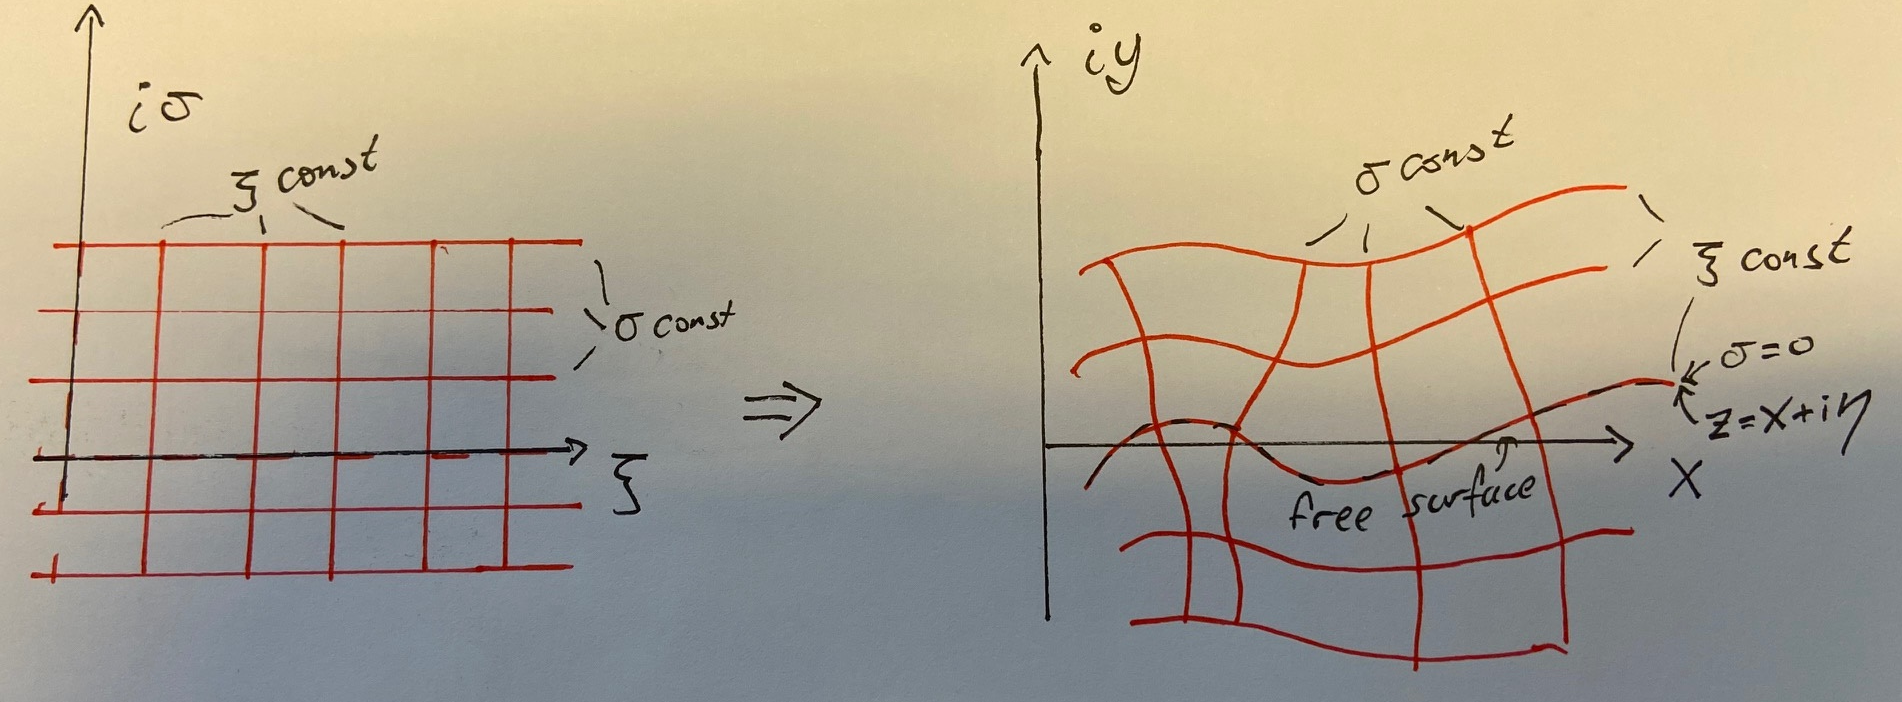
\includegraphics[width=.75\columnwidth]{./figures/map.png}%
\caption{Conformal map, mapping line $\yy=0$ to the free surface $\y=\surf$.}%
\label{fig:map}%
\end{figure}
\begin{figure}[h!ptb]%
\centering
\includegraphics[width=.75\columnwidth]{./conformal.pdf}%
\caption{The map \eqref{eq:map} in the physical $\z$-plane when $\eta(\x)$ is a single harmonic of wavenumber $\pi/2$ and amplitude $0.1$.}%
\label{fig:mapReg}%
\end{figure}

The aim of this mapping is to allow for evaluation of potential function gradients at the free surface. 
To this endeavour, we project a complex potential filed from the rectangular $\zz$-plane onto the physical $\z$-plane,
\begin{equation}
%\w(\z) = \ww[\zz(\z)],
\w(\z) = \ww[\zzmap(\z)].
\label{eq:wProj}
\end{equation}
A complex potential is defined
\[ \ww(\zz) = \phi(\xx,\yy) + \ii \psi(\xx,\yy), \]
$\phi$ being the potential function and $\psi$ the stream function in the rectangular plane.
%We have available the free surface values of the potential function $\phi\S(x)$ and so the function matching is
We have available the potential $\phi\S(\x)$ at the free surface of the physical $\z$-plane, which constitutes the line $\yy=0$ in the rectangular  $\zz$-plane. 
Accordingly, we match the functions
\begin{equation}
%\Re \w(x+\ii\surf) = \Re \ww(x) = \phi\S(x).
\phi\S(\x) = \Re \w(\x+\ii\surf) = \Re \ww[\zzmap(\x+\ii\surf)] = \Re \ww(\x).
\label{eq:wMatch}
\end{equation}
Equations \eqref{eq:invMap} and \eqref{eq:wProj} were here invoked to demonstrate the matching.
The deep water
%\footnote{In intermediate depth $h$, $\ww(\zz) = \sum_{j=0}^\infty a_j \frac{\sin k_j(\zz+\ii h)}{\cosh k_j h}$.}
 complex potential is in the rectangular plane defined as a combination of positive wavenumber Fourier modes
\begin{equation}
\ww(\zz) = \sum_{j=0}^\infty \h\ww_j \ee^{-\ii k_j \zz}; \quad k_j\geq 0
\label{eq:w}
\end{equation} 
that decay in the positive $\yy$ direction.
Matching condition \eqref{eq:wMatch} yields
\begin{equation}
\h\ww_0 = \h\phi_0\S, \quad \h\ww_j = 2\big(\h\phi\S_j\big)^*;\; j>0, 
\label{eq:aj}
\end{equation}
$\{\h\phi\S_j\}$ being the Fourier components of $\phi\S(x)$ and asterisk denoting the complex conjugate.

We now have the ingredients necessary to compute the velocities $U=u+\ii v$ at the free surface. 
The chain rule yields
\begin{equation*}
%U^* = \dd{\w}{\z}\bigg|_{0} = \dd{}{\z}\ww[\zz(\z)]\bigg|_0 = \dd\ww\zz\dd\zz\z\bigg|_0 = \bigg(\dd\ww\zz\bigg|_0\bigg)\bigg(\dd\z\zz\bigg|_0\bigg)^{-1},
U_0^* = \dd{\w}{\z}\bigg|_{0} = \dd{}{\z}\ww[\zzmap(\z)]\bigg|_0 = \ww'/\zmap' \big|_0,
%\label{eq:U_derive}
\end{equation*}
zero denoting evaluation at surface $\z=\x+\ii\surf$, $\zz=\xx$.
Inserting \eqref{eq:map} and \eqref{eq:w}, the full expression becomes
\begin{equation}
U^*(\x+\ii\surf) = \frac{1}{\ii- \surf_{\x}}\sum_{j=0}^\infty  k_j \h\ww_j \ee^{-\ii k_j \x},
\label{eq:U}
\end{equation}
with, of course, $\surf_\x=\sum_{j=-\infty}^\infty\ii k_j\h\surf_j\ee^{\ii k_j \x}$.
Expression \eqref{eq:aj} and \eqref{eq:U} is all that is needed to compute the vertical velocity at the surface in deep water. Written in terms of efficient FFT and iFFT algorithms:
\begin{equation}
U_j^* = \frac{-2\ii}{N} \frac{  \mr{FFT}\{k_j [\mr{FFT}(\phi_j\S)]^* \delta_{j}^+\}}{ 1-\mr{iFFT}[k_j \mr{FFT}(\eta_j)]}
\end{equation}
with $N$ being the number of points/modes and $\delta_{j}^+=1$ for $k_j>0$ and zero otherwise.
\\

We remark on the unexpected explicitness of this approach. 
Conformal mapping strategies often require inverse mapping $\zzmap$ which cannot be preformed explicitly. 
A key feature of the problem at hand is however that we only require potential function \textit{derivatives} along a prescribed path.






\section{The conformal mapping technique in finite water depth}
\label{sec:finiteDepth}
Unsurprisingly, the conformal map suggested in equation \eqref{eq:map} turns out not to be original, with similar mappings fond in e.g.~\citet{chalikov2005modeling}, although its usefulness in deep-water application in the context described above appears to be unremarked.
The deep water assumption may at first glance may look like a minor simplification, but it is in fact essential for the explicitness and simplicity of the above scheme. 
Let's look at the problems faced by a finite depth.
\\

The conformal map, equivalent to \eqref{eq:map}, with a finite water depth $H$ is
\begin{equation}
z\mapsto \zmap(\zz) = \zz - \ii \sum_{j=-\infty}^\infty \h\eta_j \frac{\ee^{\ii \kk_j(\zz+\ii H)}}{\sinh \kk_jH}.
\label{eq:map_H}
\end{equation}
This map does \textit{not} have the property \eqref{eq:mapXi} but rather
\begin{equation}
\Im \zmap(\xx) = \surf(\xx).
\label{eq:ImMapXi}
\end{equation}
The difference is that $\zmap(\xx)$ comes with a stretching of the $x$-dimension where
\begin{equation}
\Re \zmap(\xx) \equiv x\S(\xx) = \xx -\ii  \sum_{j=-\infty}^\infty \h\eta_j \frac{\ee^{\ii \kk_j\xx}}{\tanh \kk_j H}
\label{eq:mapXi2}
\end{equation}
(the latter term also being real).
This means that $\surf(\xx)$ in \eqref{eq:ImMapXi}, the surface boundary in the $\zz$-plane, is no functionally equivalent to the the surface $h(\x)$ in the physical plane, but rather
$\eta(\xx)=h[x\S(\xx)]$, and it is the Fourier components of $\eta(\xx)$, not of $h(\x)$, that are required in \eqref{eq:map_H}. 
Likewise, $\kk_j$ are the wave numbers in the $\zz$-plane, as opposed to the wavenumbers $k_j$ in the $\z$-plane.
In other words, the mapping \eqref{eq:map_H} is highly implicit in both directions.
It is easily plotted reversely---given a function $\eta$ in the $\zz$-plane we can compute the map \eqref{eq:map_H} and see what physical surface $h(x)$ this corresponds to.
An example is shown in \autoref{fig:map_H} for a sinusoidal $\eta(\xx)$. Note that the surface $h(x)$ in the physical plane is not sinusoidal.
The mapping, being impractical viewed from the $\z$-plane, can still adopt for wave simulation by reformulating the boundary problem into the $\zz$-plane and performing the time integration in Fourier-space, as done by \citet{chalikov2005modeling}.


We remark that similar to earlier we have $\zzmap[x\S(\xx)+\ii\eta(\xx)]=\xx$, etc.
The complex potential of finite depth is in the $\zz$-plane is
\begin{equation}
%\ww(\zz) = \sum_{j=0}^\infty\h\ww_j \frac{\sin k_j(\zz+\ii H)}{\cosh k_j H}; \quad \h\ww_j\in\mathbb R,\; k_j\geq 0.
\ww(\zz) = \sum_{j=-\infty}^\infty\h\ww_j \frac{\ee^{\ii \kk_j(\zz+\ii H)}}{\cosh \kk_j H}; \quad \h\ww_{-j}=\h\ww_{j}^*.
\label{eq:wH}
\end{equation}
The stretching $x\S(\xx)$ further affects the mapping of $\phi\S(\x)$ into the coefficients $\{\h\ww_j\}$.

\begin{figure}[h!ptb]%
\centering
\includegraphics[width=.75\columnwidth]{./conformalH.pdf}%
\caption{The map \eqref{eq:map_H} in the physical $\z$-plane when $\eta(\xx)$ is a single harmonic of wavenumber $\pi$ and amplitude $0.075$. $H=0.75$.}%
\label{fig:map_H}%
\end{figure}




\section{Algebraic conformal maps that emulate the presence of a discontinuous bathymetry}
\label{sec:SC}
Assume we have mapped a flat-bedded domain in the $\zz$-plane into a curvilinear $\z$ plane. 
A common example of such a mapping is the Schwarz--Christoffel  transformation $\z\mapsfrom \zmap(\zz)$ with
\begin{equation}
\zmap'(\zz) = C \prod_{j=1}^J (\zz-\xx_j)^{-\alpha_j/\pi},
\label{eq:SC}
\end{equation}
in which the horizontal coordinate is bent stiff angles $\alpha_j$ at locations $\zz=\xi_j$.
Some particular mappings are analytically integrable, such as the orthogonal step which yields
\begin{equation}
\z\mapsfrom\zmap(\zz) = \frac {H\_d-H\_s}\pi \left[  \sqrt{\zz-1}\sqrt{\zz+1} - 2\sinh^{-1}\! \sqrt{(\zz-1)/2} \right] - \ii H\_s,
\label{eq:mapSC}
\end{equation}
$H\_d$ and $H\_s$ being the deep and shallow sides of the step, respectively.%
\footnote{This is mapping the plane into $\zz_1=-1$, $\zz_2=1$. A less streched map is obtained if mapping into, say, $\zz_1=-d$, $\zz_2=0$; $d=H\_d-H\_s$, yielding
\[
\zmap(\zz) =   \frac {2d}\pi \left[  \sqrt{\zz/d}\sqrt{\zz/d+1} - \ln\left(\sqrt{\zz/d} \sqrt{\zz/d+1}\right) \right] - \ii H\_s,
\]
 }
An example of such a map is presented in \autoref{fig:SC_step}
Map \eqref{eq:mapSC} cannot be analytically inverted.
\\

\begin{figure}[H]%
\centering
\subfloat[$\z$-plane]{\includegraphics[width=.5\columnwidth]{../conformalMapping/conformalBathymetry/SC_step.pdf}}%
\subfloat[$\zz$-plane]{\includegraphics[width=.5\columnwidth]{../conformalMapping/conformalBathymetry/SC_step_inv.pdf}}%
\caption{A step mapped with the Schwarz--Christoffel transform \eqref{eq:mapSC}}%
\label{fig:SC_step}%
\end{figure}




%\section{Conformal step with flat surface $y=0$}
%\label{sec:SC_extended}



The step map displayed in \autoref{fig:SC_step} can be given a flat surface $y=0$ with some added complexity in the transformation function.
We base such a map on the common presented task of finding a flow field over a step in a channel \citep[e.g.,][\SSS 4.3.2]{mei_2005}\footnote{with opposite sign of $\lambda$ to shift the domain in $\zz$ by $-\ii\pi$.}.
The complex potential there created can itself be regarded as a conformal map.
Accordingly, we have
\begin{subequations}
\begin{align}
%\lambda &= -\exp(\zz),\label{eq:map_logstrip:lambda}\\
%\tau &= \sqrt{\frac{\lambda-c^2}{\lambda-1} },\label{eq:map_logstrip:t}\\
\lambda &= \exp(\zz),\label{eq:map_logstrip:lambda}\\
\tau &= \sqrt{\frac{\lambda+c^2}{\lambda+1} },\label{eq:map_logstrip:t}\\
z &\mapsfrom \zmap(\zz) = -\ii H\_s +\frac{H\_d}{\pi}\left[ 
\frac1c \ln^+\frac{\tau-c}{\tau+c} - \ln\frac{\tau-1}{\tau+1}
\right]\label{eq:map_logstrip:z},
\end{align}%
\label{eq:map_logstrip}%
\end{subequations}%
with $c = H\_d/H\_s$.
The map \eqref{eq:map_logstrip} goes via the map \eqref{eq:map_logstrip:lambda}, mapping $\zz$ the polar plane $\lambda$ (normally considered a stream function source), and the right angled $\tau$-plane \eqref{eq:map_logstrip:t}.
The flat-surface domain of $z=\x+\ii\y$, $\y\leq0$ is mapped by the strip $\zz=\xx+\ii\yy$, $-\pi<\yy\leq0$.
With waves present it may be necessary to evaluate $\z$ at locations $\y>0$; $\yy>0$ for which care must be taken to choose the appropriate branches of the logarithms;
%Accordingly, we have in \eqref{eq:map_logstrip} introduced in the operators $^+\!\sqrt{\phantom{\cdot} }$ and $\ln^+$, the angles of which run from $0$ to $\pi$ and $0$ to $2\pi$, respectively.  
we introduce in \eqref{eq:map_logstrip:z} the operator $\ln^+$, the angles of which runs from $0$ to $2\pi$. 
\autoref{fig:Mei_step} shows the adjusted map \eqref{eq:map_logstrip} for $-\pi\leq\yy\leq0.5$ with the intermediate planes $\lambda(\zz)$ and $\tau(\lambda)$ shown in \autoref{fig:Mei_step_lambda_t}.
Note that the free surface $\y=0$ is a straight line  $\yy=0$ in the $\zz$-plane, but that $\xx$ is contracted over the step transition.
The direction of the step is reversed by flipping the abscissa; $z\mapsfrom-f(-\zz)$.  

For numerical precision can become an issue for large real positive or real negative values of $\zz$ due to $\lambda=\exp \zz$ reaching the precision limit. This is easily circumvented by instead following the asymptote at large value; noting that $f'(\zz)=H\_d/\pi\tau$ and that $\lim_{\xi\to\infty}\tau=1$, $\lim_{\xi\to-\infty}\tau=H\_d/H\_s$, we have 
\begin{alignat*}{2}
\zmap(\zz) &= \zmap(\xi\_s)+\frac{H\_s}\pi(\zz-\xi\_s); \quad &\xi&\to-\infty,\\
\zmap(\zz) &= \zmap(\xi\_d)+\frac{H\_d}\pi(\zz-\xi\_d); & \xi&\to+\infty,
\end{alignat*}
$\xi\_s$ and $\xi\_d$ being locations suitably far away form the step on each side.
\\
\begin{figure}[H]%
\centering
\subfloat[$\z$-plane]{\includegraphics[width=.5\columnwidth]{../conformalMapping/conformalBathymetry/CCMei_step.pdf}}%
\subfloat[$\zz$-plane]{\includegraphics[width=.5\columnwidth]{../conformalMapping/conformalBathymetry/CCMei_step_inv.pdf}}%
\caption{A step mapped with adjusted Schwarz--Christoffel transform \eqref{eq:map_logstrip}}%
\label{fig:Mei_step}%
\end{figure}

\begin{figure}[H]%
\centering
\subfloat[$\lambda(\zz)$-plane]{\includegraphics[width=.37\columnwidth]{../conformalMapping/conformalBathymetry/CCMei_step_lambda.pdf}}%
\qquad
\subfloat[$\tau(\lambda)$-plane]{\includegraphics[width=.5\columnwidth]{../conformalMapping/conformalBathymetry/CCMei_step_t.pdf}}%
\caption{The intermediate maps \eqref{eq:map_logstrip:lambda} and \eqref{eq:map_logstrip:t}}%
\label{fig:Mei_step_lambda_t}%
\end{figure}


It is for many purposes desirable to include both forwards and backwards part of the step illustrated in \autoref{fig:Mei_step}.
This can be done by extending the Schwarz--Christoffel transformation with another step, although the differential equation thus obtained does not integrate into any wieldy analytical expression. 
It is possible to perform the integration numerically [section to come].
An alternative is to mirror the domain around the $\y$-axis at a suitable distance form the step.
\begin{equation}
\z\mapsfrom\tilde \zmap(\zz) = 
\begin{cases}
-\zmap(-\zz - L_\xx) - L_\x; & \xx < 0,\\
+\zmap(+\zz - L_\xx) + L_\x; & \xx>0,
\end{cases}
\label{eq:map_double}
\end{equation}
where $L_\xx$ and $L_\x=-f(-L_\xx)$ is the step half-width in the $\zz$ and $\z$ planes, respectively. 
This map will not be strictly conformal along the seam $\xx=0$, but approximately so provided there is some distance between the steps.
An demonstration is shown in \autoref{fig:Mei_double}.

\begin{figure}[H]%
\centering
\subfloat[$\z$-plane]{\includegraphics[width=.5\columnwidth]{../conformalMapping/conformalBathymetry/CCMei_doubleStep.pdf}}%
\subfloat[$\zz$-plane]{\includegraphics[width=.5\columnwidth]{../conformalMapping/conformalBathymetry/CCMei_doubleStep_inv.pdf}}%
\caption{A doubel step mapped with adjusted Schwarz--Christoffel transform \eqref{eq:map_double}}%
\label{fig:Mei_double}%
\end{figure}

%The complex potential of these flows can now in the $\zz$-plane be expressed
%\begin{equation}
%\ww(\zz) = \sum_{j=-\infty}^\infty \h\ww_j \frac{\ee^{\ii \kk_j(\zz+\ii\pi)}}{\cosh(\kk_j \pi)}; \quad \h\ww_{-j}=\h\ww_{j}^*.
%\label{eq:ww}
%\end{equation}
We remark that despite the many mapping levels of \eqref{eq:map_logstrip}, computing mapping derivatives is a manageable task:
\begin{equation}
\begin{aligned}
f'(\zz) &= \frac{H_d}{\pi\, \tau},  \\
f''(\zz) &= \frac{H_d \lambda\, \tau}{2\pi} \frac{c^2-1}{\rbr{c^2+\lambda}^2},\\
f'''(\zz) &= \frac{H_d \lambda\, \tau^3}{4\pi} \rbr{c^2\lambda - 2\lambda^2 + 2c^2-\lambda} \frac{c^2-1}{\rbr{c^2+\lambda}^4},\\
&\ldots
\end{aligned}
\label{eq:}
\end{equation}

\section{Numerically integrated conformal maps}
\label{sec:SCnum}
The Schwartz--Christoffel transform \eqref{eq:SC} is a powerful approach for imposing straight angles in a mapping.
A limitation of this approach is that the transform defines only the map differential, which is integrable only is special cases. 
One can however always perform integration numerically.
For example, a map similar to \eqref{eq:map_logstrip}, \autoref{fig:Mei_step}, but with a sloping depth transition, is computed by integrating
\begin{equation}
\zmap'(\zz) = \frac{H\_s}{\pi \tau_\theta}, \qquad \tau_\theta = \rbr{\frac{\lambda + (H\_d/H\_s)^{\pi/\theta}}{\lambda+1}}^{\theta/\pi}. 
\label{eq:SCnumStep}
\end{equation}
The path of such an integration is irrelevant since the map is conformal; we integrate from the top of the domain down to avoid spreading numerical imprecision form the singularities located at $\zeta=-\ii\pi$ and $\zeta=2\ln c-\ii\pi$ into the domain.
An example is shown on \autoref{fig:SCnumStep45deg} for a 45\textdegree down-step.

\begin{figure}[H]%
\centering
\subfloat[$\zz$-plane]{\includegraphics[width=.47\columnwidth]{../conformalMapping/conformalBathymetry/SCnumStep45deg_zz.pdf}}%
\hfill
\subfloat[$\z$-plane]{\includegraphics[width=.47\columnwidth]{../conformalMapping/conformalBathymetry/SCnumStep45deg_z.pdf}}%
\caption{Numerical integration of \eqref{eq:SCnumStep} with $\theta=\pi/4$, $H\_s = 0.5$ and $H\_d = 1.0$.}%
\label{fig:SCnumStep45deg}%
\end{figure}


We can extend this technique to combine several alterations in bathymetry level by adopting
\begin{equation}
\zmap'(\zz) = K \prod_{j=1}^{N_\angle} \rbr{\frac{\exp(\zz-\xi^\angle_j)+1}{\exp(\zz-\xx^\angle_j) + (H_{j+1}/H_j)^{\pi/\theta_j}}}^{\theta_j/\pi}
\label{eq:SCnumMultiStep}
\end{equation}
and fixing the constant $K$ after integration (re-scaling). $N_\angle$ is here the number of depth transitions, $\{H_j\}$ the set of depths, $\{\theta_j\}$ ($>0$) the slopes of the individual transitions and $\{\xi^\angle_j\}$ the horizontal position around which it occurs in the $\zz$-plane. 
The singularities of \eqref{eq:SCnumMultiStep} are found at $\zz=\xx^\angle_j-\ii \pi$ and $\zz=\xx^\angle_j+\pi/\theta_j\ln(H_{j+1}/H_j)-\ii \pi$.
\autoref{fig:SCnumStep2x45deg} shows an example similar to the plateau seen earlier. 
A rougher bathymetry is displayed in \autoref{fig:SCnumMultiStep}. 
The deformation of some of the sharp corners in this image is due to inaccuracy in the numeral integration near the singularity and is of no consequence for simulation usage.
Corners can of course be smoothened by defining a higher bathymetry level $\yy=\tilde H < \pi$ in the $\zz$-plane, as shown in \autoref{fig:SCnumMultiStepSmooth}.

\begin{figure}[H]%
\centering
\subfloat[$\zz$-plane]{\includegraphics[width=.47\columnwidth]{../conformalMapping/conformalBathymetry/SCnumStep2x45deg_zz.pdf}}%
\hfill
\subfloat[$\z$-plane]{\includegraphics[width=.47\columnwidth]{../conformalMapping/conformalBathymetry/SCnumStep2x45deg_z.pdf}}%
\caption{Numerical integration of \eqref{eq:SCnumMultiStep} with 
%$\theta_1=\theta_2=\pi/4$; $H_1 = 1.0$, $H_2 = 0.5$, $H_3 = 1.0$ and $\xi^\angle_1=0$, $\xi^\angle_1=5$.
$\theta_j\in\{\pi/4,\pi/4\}$, $H_j \in\{1.0,0.5,1.0\}$ and $\xx^\angle_j\in\{0,5\}$.
}%
\label{fig:SCnumStep2x45deg}%
\end{figure}

\begin{figure}[H]%
\centering
\subfloat[$\zz$-plane]{\includegraphics[width=.47\columnwidth]{../conformalMapping/conformalBathymetry/SCnumStepMulti_zz.pdf}}%
\hfill
\subfloat[$\z$-plane]{\includegraphics[width=.47\columnwidth]{../conformalMapping/conformalBathymetry/SCnumStepMulti_z.pdf}}%
\caption{Numerical integration of \eqref{eq:SCnumMultiStep} with 
$\theta_j\in\{\pi/4,5\pi/2,5\pi/2\}$, $H_j \in\{0.5,1.5,0.75,1.5\}$ and $\xx^\angle_j\in\{0,8,14\}$.
}%
\label{fig:SCnumMultiStep}%
\end{figure}

\begin{figure}[H]%
\centering
\includegraphics[width=.47\columnwidth]{../conformalMapping/conformalBathymetry/SCnumStepMultiSmooth_z.pdf}%
\caption{As \autoref{fig:SCnumMultiStep}, instead choosing bethymetry at $\yy = 0.1-\pi$.
}%
\label{fig:SCnumMultiStepSmooth}%
\end{figure}


\section{Generalization to a transient mapping}
%\documentclass[a4paper,12pt]{article}
%%\documentclass{amsart}
%\usepackage[a4paper, total={17cm, 25cm}]{geometry}
%\usepackage[utf8]{inputenc}
%\usepackage[english]{babel}
%\usepackage{amsmath,bm,amsfonts,amssymb}
%\usepackage{xcolor}
%\usepackage{graphicx}
%
%\usepackage{stmaryrd}
%\usepackage[round]{natbib}
%\usepackage{mathtools}
%\usepackage[font=normalsize]{subfig}
%\usepackage{float}
%\usepackage{hyperref}
%\usepackage{enumitem}
%\hypersetup{colorlinks=true, 	
			%linkcolor=blue,
			%filecolor=blue,
			%urlcolor=blue,
			%citecolor=blue}
%\newcommand{\mr}{\mathrm}
%\newcommand{\mc}{\mathcal}
%\let\SSS\S
%\renewcommand{\S}{^\mr{S}}
%\newcommand{\ii}{\mr{i}\,}
%\newcommand{\ee}{\mr{e}}
%%\newcommand{\phit}{\psi}
%\newcommand{\phit}{\tilde\phi}
%\newcommand{\br}[3]{\left#1#2\right#3}
%\let\underscore\_
%\renewcommand{\_}[1]{_\mr{#1}}
%\newcommand{\oo}[1]{^{(#1)}}
%\newcommand{\rr}{\bm r}%{x,y}
%\newcommand{\cp}{c\_p}
%\let\Re\relax
%\let\Im\relax
%\DeclareMathOperator\Re{Re}
%\DeclareMathOperator\Im{Im}
%\newcommand{\w}{w}
%\newcommand{\bU}{\bm U}
%\newcommand{\h}{\hat}
%\newcommand{\rbr}[1]{\left(#1\right)}
%\newcommand{\sbr}[1]{\left[#1\right]}
%\newcommand{\cbr}[1]{\left\{#1\right\}}
%\newcommand{\z}{z}
%\newcommand{\x}{x}
%\newcommand{\y}{y}
%\newcommand{\zz}{\zeta}
%\newcommand{\xx}{\xi}
%\newcommand{\yy}{\sigma}
%%\newcommand{\k}{k}
%\newcommand{\kk}{\kappa}
%
%
%\newcommand{\zmap}{f}
%%\newcommand{\zzmap}{\zmap^{-1}}
%\newcommand{\zzmap}{\zmap^{\raisebox{.2ex}{$\scriptscriptstyle-1$}}}
%
%\newcommand{\ww}{\omega}
%\renewcommand{\w}{w}
%\newcommand{\surf}{\eta}
%\newcommand{\dd}{\mr d}
%\newcommand{\ddfrac}[2]{\frac{\dd #1}{\dd #2}}
%
%\begin{document}










Let us assume that our mapping is time dependent, i.e.,
\begin{equation}
z \mapsfrom f(\zz,t).
\label{eq:}
\end{equation}
Such a map can for example account for the action of a wavemaker on the body of water.
We now derive the associated system equations in terms of $\zz$-variables.
The kinematic boundary condition states that a fluid particle follows the surface, also in the $\zz$-plane.
This can be expressed by $\frac{\mr D}{\mr Dt}(\eta_{\xx,t}-\yy)=0$ where
the material derivative velocity $\UU=\ddfrac{\zz\_p}{t}$ as seen from the $\zz$-plane:
%\[
%\UU = \ddfrac{\zz\_p}{t} = (\zzmap)_z \ddfrac{\z\_p}{t} + (\zzmap)_t = \frac{\w_z^*}{\zmap_\zz} + (\zzmap)_t =  \frac{\ww_\zz^*}{|\zmap_\zz|^2} + (\zzmap)_t,
%\]
\[
\ddfrac{\z\_p}{t} = \zmap_\zz \UU + \zmap_t
\]
subscript `p' indicating fluid particle position.
Fluid particles are advected with the the flow velocity of the $\z$-plane, $\ddfrac{\z\_p}{t}=\w_\z^*=(\ww_\zz/\zmap_\zz)^*$.
We accordingly get
\begin{equation}
\UU = \frac{\ww_\zz^*}{\Jac}-\frac{\zmap_t}{\zmap_\zz},
\label{eq:UU}
\end{equation}
and the kinematic boundary condition
\begin{equation}
\eta_t = - \Re \UU \eta_\xx + \Im \UU,
\label{eq:BC_kin_transientU}
\end{equation}
or, written in terms of the surface potential $\varphi\S(\xx,t)=\varphi[\xx,\eta(\xx,t),t]$,
\begin{equation}
\eta_t = \iJac\sbr{\varphi_\yy\rbr{1+\eta_\xx^2}-\varphi\S_\xx} + \eta_\xx \Re\rbr{\frac{\zmap_t}{\zmap_\zz}}-\Im\rbr{\frac{\zmap_t}{\zmap_\zz}}.
\label{eq:BC_kin_transient}
\end{equation}
%
%The kinematic condition requires an the inverse map time derivative $(\zzmap)_t$. 
%Utilizing the property $(\zzmap)_\z = 1/\zmap_\zz$, we find
%\begin{equation}
%(\zzmap)_t = \int \!\big(1/\zmap_\zz\big)_t \,\dd z = -\int\! \frac{\zmap_{\zz t}}{\zmap_\zz} \,\dd\zz.
%\label{eq:zzmap_t}
%\end{equation}
%Integrating \eqref{eq:zzmap_t} is the same challenge as we face with the Schwartz--Cristoffel transform where
%analytic expressions exist for some maps but not all. Numerical integration can be performed where analytic expressions are not forthcoming. 
\\

Deriving the dynamic boundary condition is straight-forwart when adopting the complex potentials $\ww(\zz,t)=\w[\zmap(\zz,t),t]$; $\phi=\Re\w$, $\varphi = \Re\ww$.
This yields
\begin{equation}
\varphi_t = \Re\sbr{\ww_\zz \frac{\zmap_t}{\zmap_\zz}} - \frac12\iJac|\ww_\zz|^2 - gh.
\label{eq:}
\end{equation}
Further introducing $\varphi\S(\xx,t)=\varphi[\xx,\eta(\xx,t),t]$ to eliminate $\varphi_t$ and $\varphi_\xx$, we get 
\begin{equation*}
\varphi\S_t =\Re\sbr{\ww_\zz \frac{\zmap_t}{\zmap_\zz}} + \varphi_\yy \eta_t
 - \frac12\iJac\sbr{\rbr{\varphi\S_\xx-\varphi_\yy\eta_\xx}^2+\varphi_\yy^2} - gh.
\end{equation*}
%
Eliminating $\eta_t$ with \eqref{eq:BC_kin_transient} finally produces
%\begin{equation}
%\varphi\S_t - \Re\sbr{\ww_\zz \frac{\zmap_t}{\zmap_\zz}}
%+ \varphi_\yy\sbr{\Re(\zzmap)_t-\eta_\xx\Im(\zzmap)_t}
 %+ \frac12\iJac\sbr{\rbr{\varphi\S_\xx}^2-\rbr{1+\eta_\xx^2}\varphi_\yy^2} + gh = 0.
%\label{eq:BC_dyn_transient}
%\end{equation}
\begin{equation}
\varphi\S_t =  \varphi\S_\xx \Re\rbr{ \frac{\zmap_t}{\zmap_\zz}}
 - \frac12\iJac\sbr{\rbr{\varphi\S_\xx}^2-\rbr{1+\eta_\xx^2}\varphi_\yy^2} - gh.
\label{eq:BC_dyn_transient}
\end{equation}
\\

An example of a Schwartz-Christoffel type transform of a flap wavemaker is
\begin{equation}
\zmap_\zz(\zz,t) = \prod_{j=-\infty}^\infty \rbr{1+\frac{d^2}{\rbr{\zz+2\ii j h}^2}}^{\theta(t)/\pi}
= \sbr{1+\frac{\sin^2\!\frac{\pi d}{2h}}{\sinh^2\!\frac{\pi \zz}{2h}}}^{\theta(t)/\pi}
\label{eq:df_flap}
\end{equation}
This map is a $\theta$-bend in the vertical axis mirrored about the horizontal axis.
This is then mirrored again infinitely many times for every $2\ii h$-period---a product series which expressible in terms of trigonometric functions.
\eqref{eq:df_flap} is unfortunately to our knowledge not integrable, so integration must be carried out numerically. 
We note that $\zmap_\zz\to1$ as $\xx\to\infty$ and so the $\z$ plane will scale with the $\zz$ plane far away from the wavemaker, and the two planes will match everywhere for $\theta=0$. $\zz=-\ii d$, which is the hinge position in the $\zz$-plane, will be in proximity to the hinge position in the $\z$-plane, but will shifted vertically with extending flap angles. We perform a numerical iteration in order to determine the value of $d$ to achieve the descried hinge depth $D$ in the physical plane. This is done by measuring the distance from the bottom to the hinge;
let
\begin{equation}
\mc L(d/h,\theta) = \int_{-1}^{-d/h} \dd \yy \sbr{1-\frac{\sin^2\!\frac{\pi}{2}\frac{d}{h}}{\sin^2\!\frac{\pi}{2}\yy}}^{\theta/\pi} = \frac{f(-\ii d)-f(-\ii h)}h
\label{eq:L}
\end{equation}
We iterate by assigning
\[
d\leftarrow d + h(1-\mc L) - D.
\]
Note that this makes both $d$ and $\theta$ time dependent functions.
 
The map here given has a horizontal line of symmetry along $\y=0$. The wavemaker forms a wedge at this level. 
For this not to interfare with the water level, we propose shifting the waterline down a small distance $\y=-\hbar$.
This is easily done by substituting 
%\begin{align*}
%h &\leftarrow h + \hbar, & D &\leftarrow D + \hbar, & \z &\leftarrow \z + \ii \hbar.
%\end{align*}
$h \leftarrow h + \hbar$, $D \leftarrow D + \hbar$ and $\z \leftarrow \z + \ii \hbar$, right-hand side lengths being lengths with respect to the waterline.
\\

\autoref{fig:f_flap} shows an example of \eqref{eq:df_flap} integrated numerically.
%We note that the floor near the wavemaker is with this map somewhat distorted which will cause some error in non-deep water.
\\
\begin{figure}[h!ptb]%
\centering
\subfloat[$\theta = +30$\textdegree]{\includegraphics[width=.5\columnwidth]{../conformalMapping/conformalWavemaker/mapFlap3_positive.pdf}}%
\subfloat[$\theta = -30$\textdegree]{\includegraphics[width=.5\columnwidth]{../conformalMapping/conformalWavemaker/mapFlap3_negative.pdf}}%
\caption{The conformal map \eqref{eq:df_flap}, integrated numerically.
$D=1.0$, $h=2.0$ and $\hbar = 0.25$.
}%
\label{fig:f_flap}%
\end{figure}



We may for deep water ignore the periodic mirroring in \eqref{eq:df_flap}.
This expression is integrable in terms of the  ordinary hypergeometric function ${_2F}_1$:
\begin{equation}
\tilde\zmap(\zz,t) = \int\!\dd\zz\rbr{1+\frac{b^2}{\zz^2}}^{\theta(t)/\pi}=\frac{d}{1-2\frac\theta\pi}\,{_2F}_1\rbr{-\frac{\theta}{\pi},\frac12-\frac{\theta}{\pi},\frac32-\frac{\theta}{\pi},-\frac{\zz^2}{d^2}}\rbr{\frac{\zz}{d}}^{1-2\frac\theta\pi} + c.
\label{eq:f_flap}
\end{equation}
%Equation \ref{eq:df_flap} can be integrated numerically if the hypergeometric functions are not available.\footnote{${_2F}_1$ is in MATLAB only part of the symbolic toolbox.}

The condition that the flap hinge depth be a vertical distance $D$ from the quiescent waterline at $\x=0$, and that the map return be unaffected by the wavemaker motion far away ($\lim_{\xx\to\infty}\zmap(\xi,t) = \xi$) yields the coefficients
\begin{align*}
%c &= -(D+\hbar)\tan\theta + \ii \hbar,&
%d &=  \frac{\sqrt\pi(D+\hbar)\sec\theta}{\Gamma\rbr{1+\frac\theta\pi}\Gamma\rbr{\frac12-\frac\theta\pi}}.
c = -D\tan\theta,\qquad
d =  \frac{\sqrt\pi D\sec\theta}{\Gamma\rbr{1+\frac\theta\pi}\Gamma\rbr{\frac12-\frac\theta\pi}}.
\end{align*} 
$\hbar$ is here the distance from the quiescent waterline to the line of symmetry around which the map is horizontally mirrored.

%Expression \eqref{eq:zzmap_t} is integrable with for the non-mirrored domain, producing
%\begin{equation*}
%(\tilde\zzmap)_t = -\sbr{2d\arctan\frac\zz d + \zz \ln\rbr{1+\frac{d^2}{\zz^2}}}\frac{\theta_t}{\pi}.
%\end{equation*}
%It is also integrable with \eqref{eq:df_flap} itself, although the expression we get is a mess not quoted here. 


%\end{document}


\bibliographystyle{plainnat} % abbrvnat,plainnat,unsrtnat
\bibliography{../sintef_bib} %You need a file 'literature.bib' for this.


\end{document}
